\section{Spatial spreading via transversal invasion waves}
\label{s:nonscalar-waves}

In simple monostable examples like rabies \cite{ruan2017spatiotemporal}, $R_0>1$ is equivalent to instability of the disease-free state and to invasion at positive speed. In general, for a spatially homogeneous resident with an irreducible transverse block, $R_\Sigma>1$ is equivalent to positive linear spreading speed; nonlinear invasion can also occur when $R_\Sigma<1$.

The transverse Jacobian block of a siphon face is Metzler, so the Freidlin--G\"artner--Weinberger--Lewis--Li formula gives the spreading speed of the linearized invasion equation. Identifying this speed with that of the nonlinear system requires additional linear-determinacy hypotheses.

%=======================================================================
\subsection{The transversal invasion wave optimization problem}
\label{s:opt}


\beP[Optimization formula for the linear spreading speed]
\label{t:spread}\label{p:LinSpread}
Let $\mathcal D=\diag(d_i)$ with $d_i\ge0$, not all zero, let $M$ be an irreducible Metzler matrix with $s(M)>0$, and consider
\[
 Z_t=\mathcal D\Delta_\zeta Z+MZ,\qquad Z=(Z_1,\ldots,Z_m)^\top,\quad\zeta\in\mathbb R^n.
\]
For $\lambda>0$, let $A(\lambda)=\lambda^2\mathcal D+M$, with right Perron vector $q(\lambda)\gg0$, and let $g(\lambda)=s(A(\lambda))$, $c(\lambda)=g(\lambda)/\lambda$. Then:
\begin{enumerate}
\item The function $g$ is strictly convex, and $c$ has a unique minimizer $\lambda_*>0$. Put $c_*=c(\lambda_*)>0$.
\item The number $c_*$ is the spreading speed of this linear system: for nonzero $Z(0,\cdot)\in C_c(\mathbb R^n;\mathbb R_+^m)$,
\[
 c>c_*\implies\sup_{|\zeta|\ge ct}\|Z(t,\zeta)\|\to0,\qquad
 0<c<c_*\implies\inf_{|\zeta|\le ct}Z_i(t,\zeta)\to+\infty\quad\text{for every }i .
\]
\item For every unit vector $e$ and every $\lambda>0$, $Z=e^{-\lambda(e\cdot\zeta-c(\lambda)t)}q(\lambda)$ is a solution: an exponential traveling mode normal to $e$ with speed $c(\lambda)$, unbounded behind its leading edge, so not a front joining two equilibria. The speeds of such modes are exactly the $c\ge c_*$.
\item If $p_*,q_*$ are the left and right Perron vectors of $A(\lambda_*)$, with $\langle p_*,q_*\rangle=1$, then
\[
 c_*=2\lambda_*\langle p_*,\mathcal Dq_*\rangle.
\]
\end{enumerate}
\eeP

\beR[Next-generation reading, and direction]
\label{r:splitDir}
This is the linear speed of Weinberger, Lewis and Li \cite{WeinbergerLewisLi2002}. 1. The speed of exponential modes depends in principle on $e$, but since the Laplacian
models diffusion independent of the direction, here it does not depend on $e$ (if each species $i=1,\ldots,m$ diffuses as $\nabla\cdot(\mathcal A_i\nabla Z_i)$, with $\mathcal A_i$ a constant symmetric positive definite $n\times n$ matrix, then the $m\times m$ diagonal matrix with entries $e^\top\mathcal A_1e,\ldots,e^\top\mathcal A_me$ replaces $\mathcal D$).

2. For any regular splitting $M=F-V$, $s(M)>0\iff R_0=\rho(FV^{-1})>1$.
Thus, $c_*>0$ exactly when $R_0>1$; for $s(M)<0$ the infimum is $-\infty$, and for $s(M)=0$ it is zero. For $m=1$ and $M=r$ the proposition gives the famous Fisher--KPP speed $c_*=2\sqrt{\mathcal Dr}$,
and if $r=\mu(R_0-1)$ then $c_*=2\sqrt{\mathcal D\mu(R_0-1)}$. The review \cite{DavydovychDutkaCherniha2023} surveys this dichotomy for epidemic models, from the plague and rabies models of Noble and of K\"all\'en and Murray to spatial COVID-19 models simulated in the plane with data from Lombardy.

%3. The function $g$ is convex, but $c$ need not be: for $\mathcal D=\diag(1/10,1)$ and $M=\begin{pmatrix}1&1/20\\1/20&-1\end{pmatrix}$, numerically $c''<0$ near $\lambda\approx1.8$. What holds is that the sets $\{c\le t\}=\{g-t\lambda\le0\}$ are intervals.

\eeR

\begin{proof}
(1) The Perron root of a Metzler matrix is a nondecreasing convex function of its diagonal entries, a classical fact, so $G(\mu)=s(M+\mu\mathcal D)$ is convex. Since $M$ is irreducible, $G$ is a simple eigenvalue, hence
smooth, with $G'=\langle p,\mathcal Dq\rangle>0$, because $p,q\gg0$ and $\mathcal D\ne0$. Thus $g(\lambda)=G(\lambda^2)$ has $g'=2\lambda G'$ and $g''=2G'+4\lambda^2G''\ge2G'(0)>0$. Since $g\to s(M)>0$ as $\lambda\to0^+$ and
$g\sim\lambda^2\max_id_i$, $c\to+\infty$ at both ends. A critical point of $c$ solves $h=0$ with $h=\lambda g'-g$, and $h'=\lambda g''>0$, so it is unique and is the minimizer.

(4) $c'(\lambda_*)=0$ reads $\lambda_*g'(\lambda_*)=g(\lambda_*)$.

(3) The first statement follows by substitution, and the second because $c$ is continuous with minimum $c_*$ and tends to $+\infty$.

(2) The solution operator is positive, so it suffices to bound $Z$ from below for data $\phi\in C_c^\infty(\mathbb R^n;\mathbb R_+^m)$, $\phi\ne0$, $\phi\le Z(0,\cdot)$. Then
\[
 Z(t,\zeta)=\frac1{(2\pi)^n}\int_{\mathbb R^n}e^{ik\cdot\zeta}e^{t(M-(k\cdot k)\mathcal D)}\hat\phi(k)\,dk ,
\]
where $\hat\phi$ is entire and decays rapidly on every shifted contour. Extend $g$ evenly to $\lambda\in\mathbb R$; since $g''\ge2G'(0)>0$, for each $v$ there is a unique $\lambda_v$ with $g'(\lambda_v)=v$. Put $\psi(v)=g(\lambda_v)-v\lambda_v$. For a unit vector $e$
and $\zeta=vte$, shift the contour to $k=\eta+i\lambda_ve$ and write $\eta=\eta_1e+\eta_\perp$. Then $-k\cdot k=\lambda_v^2-|\eta|^2-2i\lambda_v\eta_1$, and the matrix $M+(\lambda_v^2-|\eta|^2)\mathcal D$ is Metzler, so entrywise
\[
 \bigl|e^{t(M-(k\cdot k)\mathcal D)}\bigr|\le e^{t(M+(\lambda_v^2-|\eta|^2)\mathcal D)} ,
\]
by the Trotter product formula, the imaginary part being diagonal. The exponential of a Metzler matrix increases with its diagonal, so for $|\eta|\ge\eta_0>0$ this is at most $e^{t(M+(\lambda_v^2-\eta_0^2)\mathcal D)}\le C\,e^{tG(\lambda_v^2-\eta_0^2)}$, with $C$ uniform for $v$ in compact intervals. Since $G$ is strictly increasing, the integrand there is at most $Ce^{t(g(\lambda_v)-\delta)}|\hat\phi|$, with $\delta>0$, and $\hat\phi$ makes this part integrable; no decay in $\eta$ is needed from the diffusion. For small $\eta$ the other eigenvalues stay below $g(\lambda_v)-\delta$ in real part, and, expanding the
simple Perron eigenvalue, the linear imaginary term cancels against $e^{i\eta_1vt}$, and Laplace's method gives
\[
 Z(t,vte)=\frac{e^{t\psi(v)}}{\sqrt{2\pi t\,g''(\lambda_v)}\,(4\pi t\langle p_v,\mathcal Dq_v\rangle)^{(n-1)/2}}\Bigl(q_v\int_{\mathbb R^n}e^{\lambda_ve\cdot y}\,p_v^\top\phi(y)\,dy+o(1)\Bigr),\qquad p_v^\top q_v=1,
\]
uniformly for $v$ in compact intervals and for $e$. The integral is positive and $q_v\gg0$. Finally $\psi'(v)=-\lambda_v$, so $\psi$ is even and strictly decreasing for $v>0$, with $\psi(c_*)=0$ and $\psi(v)>0$ for $|v|<c_*$, and the exponential rate dominates the power of $t$;
this proves the interior assertion. The exterior assertion follows by comparison with the solution $Kq(\lambda)e^{-\lambda e\cdot\zeta+g(\lambda)t}$, with $e=\zeta/|\zeta|$ and $K$ independent of $e$, for a $\lambda>0$ with $c(\lambda)<c$.
\end{proof}
The formula for the derivative of a Perron eigenvalue used in the proof is classical \cite{Seneta,ElsnerJohnson,Nussbaum1986}; it also underlies the reduction principle and the evolution of dispersal \cite{Karlin1982,Altenberg2012,Dockery1998}.





\beR[A moving-frame next-generation test and a drift threshold]
\label{r:movNGM}
With the splitting $M=F-V$ of Remark~\ref{r:splitDir}, the speed can be read as a family of next-generation tests.
\begin{enumerate}
\item \emph{A moving observer; no transport is added to the model.} With $\xi=e\cdot\zeta-ct$, a perturbation $e^{-\lambda\xi}w(t)$ of the system of Proposition~\ref{t:spread} satisfies $w_t=(\lambda^2\mathcal D+F-V-c\lambda I)w$, so it decays, as seen by an observer moving at speed $c$, exactly when $s(\lambda^2\mathcal D+F-V-c\lambda I)<0$. When $B_c(\lambda)=V+c\lambda I-\lambda^2\mathcal D$ is a nonsingular $M$-matrix, the regular splitting $F-B_c(\lambda)$ turns this into $R_c(\lambda)=\rho(FB_c(\lambda)^{-1})<1$; otherwise $s(\lambda^2\mathcal D+F-V-c\lambda I)\ge0$. Hence
\[
 c>c_*\iff R_c(\lambda)<1\ \text{ for some admissible }\lambda>0:
\]
a speed exceeds $c_*$ exactly when an exponentially decaying bound of the leading edge exists in that moving frame. The value $R_c(\lambda)$ depends on the mode; it is a test, not a new reproduction number, and $R_0$ is its value at $\lambda=0$, for every $c$.
\item \emph{Near the threshold.} For a smooth family $M\to M_0$, with $M_0$ irreducible Metzler, $s(M_0)=0$, and $\mathcal D\ne0$ fixed, $c_*=2\sqrt{\langle\mathcal D\rangle\,s(M)}\,(1+o(1))$, where $\langle\mathcal D\rangle=p^\top\mathcal Dq/p^\top q$ with $p,q$ the Perron vectors of $M_0$.
\item \emph{Physical drift.} Consider $Z_t=dZ_{\zeta\zeta}+qZ_\zeta+(b-v)Z$ with $d>0$, $b>v>0$, $q\ge0$: the transport is toward decreasing $\zeta$, $R_0=b/v$, the speed against the flow is $c_{\rm up}=2\sqrt{d(b-v)}-q$, and
\[
 R_{\rm abs}=\min_{\substack{\lambda\ge0\\v+q\lambda-d\lambda^2>0}}\frac b{v+q\lambda-d\lambda^2}=\frac b{v+q^2/(4d)},\qquad R_{\rm abs}>1\iff q<2\sqrt{d(b-v)}.
\]
In the range $R_{\rm abs}<1<R_0$ the perturbation grows but cannot spread upstream \cite{SpeirsGurney2001}. In general, for $Z_t=\mathcal D\Delta_\zeta Z+Q\,\nu\cdot\nabla_\zeta Z+MZ$, with $Q\ge0$ diagonal and $\nu$ a fixed unit vector, the matrix $\lambda^2\mathcal D-\lambda(e\cdot\nu)Q+M$ depends on $e$. For $e=\nu$, let $c_{\rm up}=\inf_{\lambda>0}s(\lambda^2\mathcal D-\lambda Q+M)/\lambda$ and let $R_{\rm abs}$ be the infimum of $\rho(F(V-\lambda^2\mathcal D+\lambda Q)^{-1})$ over $\lambda\ge0$ with $V-\lambda^2\mathcal D+\lambda Q$ a nonsingular $M$-matrix. Then $R_{\rm abs}>1$ implies $c_{\rm up}>0$, and $c_{\rm up}>0$ implies $R_{\rm abs}\ge1$, strictly when the infimum is attained. For $Q=qI$, $c_{\rm up}=c_*-q$.
\end{enumerate}
All this concerns the linear speed: when growth is stronger at higher density, a front can advance although $R_0<1$.
\eeR

\beR[Linear invasion speeds on the siphon lattice]
\label{ss:kpp-siphon}
Let $P_\Sigma$ be a spatially constant resident equilibrium on a siphon face, with irreducible transverse matrix $M=F_\Sigma(P_\Sigma)-V_\Sigma(P_\Sigma)$, $s(M)>0$ and $\mathcal D_\Sigma\ne0$. Proposition~\ref{t:spread} then gives the linear spreading speed
\[
 c_\Sigma(P_\Sigma)=\inf_{\lambda>0}\frac1\lambda\,s\bigl(\lambda^2\mathcal D_\Sigma+F_\Sigma(P_\Sigma)-V_\Sigma(P_\Sigma)\bigr).
\]
Reducible blocks and spatially varying residents require further analysis.
In multistrain systems this gives $c_1,c_2$ for the linearized invasion of the disease-free equilibrium by each strain, and $c_{2|1},c_{1|2}$ for the linearized invasion of the resident of the other strain.
Identifying these with the speeds of the nonlinear system requires linear-determinacy hypotheses \cite{WeinbergerLewisLi2002}; for partly diffusing cooperative systems see \cite{Li2012}.
\eeR

\subsection{Application to a two-strain cholera model}
\label{ss:kpp-two-strain}

\beF[Species-reaction graph of a two-strain cholera model]
\centering
\begin{tikzpicture}[>=stealth, scale=1.0,
  species/.style={rectangle, draw, thick,
                  minimum width=1.1cm, minimum height=0.65cm},
  rxn/.style   ={circle, draw, thick, fill=white,
                  font=\small, inner sep=3pt},
  sp2rx/.style ={->, dotted, thick},
  rx2sp/.style ={->, dashed, thick}
]

%% ── Left panel: ODE system ────────────────────────────────────────
\node[anchor=north west, inner sep=0pt] at (0, 0.3) {%
  % 5.6cm was 18.8pt too narrow for the S_t line; the right panel begins at
  % xshift=8.2cm with its leftmost arrow at 6.6cm, so 6.3cm still clears it.
  \parbox{6.3cm}{%
    \[
    \left\{
    \begin{aligned}
    S_t      &= \Lambda-\mu S-\beta_1SB_1-\beta_2SB_2,\\
    (I_1)_t  &= \beta_1SB_1-(\mu+\gamma_1)I_1,\\
    (I_2)_t  &= \beta_2SB_2-(\mu+\gamma_2)I_2,\\
    (B_1)_t  &= d_1\Delta_\zeta B_1+\xi_1I_1-\delta_1B_1,\\
    (B_2)_t  &= d_2\Delta_\zeta B_2+\xi_2I_2-\delta_2B_2.
    \end{aligned}
    \right.
    \]%
  }%
};

%% ── Right panel: CRN graph ────────────────────────────────────────
\begin{scope}[xshift=8.2cm, scale=0.90]

%% Species
\node[species] (S)  at (0,    0)   {$S$};
\node[species] (I1) at (3,  1.8)   {$I_1$};
\node[species] (I2) at (3, -1.8)   {$I_2$};
\node[species] (B1) at (6,  1.8)   {$B_1$};
\node[species] (B2) at (6, -1.8)   {$B_2$};

%% Bipartite reaction nodes — infection
\node[rxn] (R3) at (1.5,  1.8) {\scriptsize$\beta_1 SB_1$};
\node[rxn] (R4) at (1.5, -1.8) {\scriptsize$\beta_2 SB_2$};

%% Bipartite reaction nodes — shedding (offset above/below to avoid overlap)
\node[rxn] (R7) at (4.5,  2.7) {\scriptsize$\xi_1 I_1$};
\node[rxn] (R8) at (4.5, -2.7) {\scriptsize$\xi_2 I_2$};

%% Linear inflows / outflows
\draw[->] (-1.6, 0)    -- (S)            node[midway, above] {$\Lambda$};
\draw[->] (S.north)    -- ++(0,+0.9)     node[above]         {$\mu S$};
\draw[->] (I1.north)   -- ++(0,+0.9)     node[above]         {$(\mu{+}\gamma_1)I_1$};
\draw[->] (I2.south)   -- ++(0,-0.9)     node[below]         {$(\mu{+}\gamma_2)I_2$};
\draw[->] (B1.north)   -- ++(0,+0.9)     node[above]         {$\delta_1 B_1$};
\draw[->] (B2.south)   -- ++(0,-0.9)     node[below]         {$\delta_2 B_2$};

%% Infection reactions (strain 1)
\draw[sp2rx] (S.north east) to[bend left=20]  (R3);
\draw[sp2rx] (B1.west)                       -- (R3);
\draw[rx2sp] (R3)                             -- (I1);

%% Infection reactions (strain 2)
\draw[sp2rx] (S.south east) to[bend right=20] (R4);
\draw[sp2rx] (B2.west)                       -- (R4);
\draw[rx2sp] (R4)                             -- (I2);

%% Shedding reactions (strain 1): I_1 -> I_1 + B_1
\draw[sp2rx] (I1.north) to[bend left=15]   (R7);
\draw[rx2sp] (R7)       to[bend left=15]   (I1.east);
\draw[rx2sp] (R7)       to[bend right=15]  (B1.north);

%% Shedding reactions (strain 2): I_2 -> I_2 + B_2
\draw[sp2rx] (I2.south) to[bend right=15]  (R8);
\draw[rx2sp] (R8)       to[bend right=15]  (I2.east);
\draw[rx2sp] (R8)       to[bend left=15]   (B2.south);

\end{scope}
\end{tikzpicture}

\vspace{0.8em}
\renewcommand{\arraystretch}{1.2}
\begin{tabular}{rllp{5.2cm}}
\toprule
No. & Reaction & Rate & Interpretation \\
\midrule
1  & $\varnothing\to S$       & $\Lambda$               & Host recruitment \\
2  & $S\to\varnothing$        & $\mu S$                 & Natural death of $S$ \\
3  & $S+B_1\to I_1+B_1$      & $\beta_1 SB_1$          & Strain-1 infection ($B_1$ catalytic) \\
4  & $S+B_2\to I_2+B_2$      & $\beta_2 SB_2$          & Strain-2 infection ($B_2$ catalytic) \\
5  & $I_1\to\varnothing$      & $(\mu+\gamma_1)I_1$     & Removal of infected host $I_1$ \\
6  & $I_2\to\varnothing$      & $(\mu+\gamma_2)I_2$     & Removal of infected host $I_2$ \\
7  & $I_1\to I_1+B_1$        & $\xi_1 I_1$             & Pathogen shedding by $I_1$ ($I_1$ catalytic) \\
8  & $I_2\to I_2+B_2$        & $\xi_2 I_2$             & Pathogen shedding by $I_2$ ($I_2$ catalytic) \\
9  & $B_1\to\varnothing$      & $\delta_1 B_1$          & Environmental decay of $B_1$ \\
10 & $B_2\to\varnothing$      & $\delta_2 B_2$          & Environmental decay of $B_2$ \\
\bottomrule
\end{tabular}
\lbl{fig:twostrain-env}
\caption{Two-strain environmental transmission model.
  \emph{Left}: ODE/PDE system (\textbf{diffusing}: $B_1, B_2$;
  \textbf{non-diffusing}: $S, I_1, I_2$).
  Disease siphons: $\sigma_k=\{I_k,B_k\}$, $k=1,2$,
  and the joint siphon $\sigma_{12}=\{I_1,B_1,I_2,B_2\}$.
  \emph{Right}: species-reaction (Volpert/DSR hybrid) graph.
  All multi-species reactions are shown as bipartite nodes.
  Infection reactions~3--4 ($S+B_k\to I_k+B_k$): dotted arrows from
  $S$ and $B_k$ into the node, dashed arrow out to $I_k$.
  Shedding reactions~7--8 ($I_k\to I_k+B_k$): dotted arrow from $I_k$
  into the node, dashed arrows out to $I_k$ (returned) and $B_k$
  (produced); nodes placed above/below the species row to avoid overlap.
  \textbf{Dotted}: reactant $\to$ node;
  \textbf{dashed}: node $\to$ product.}
\eeF
%%%%%%
The disease-free equilibrium is
$$
X_0=
\left(
\frac{\Lambda}{\mu},
0,0,0,0
\right).
$$

The strain-$1$ transversal subsystem at the DFE is
$$
Z_1=(I_1,B_1)^T,
$$
with
$$
(Z_1)_t
=
\mathcal D_1\Delta_\zeta Z_1
+
\T M_1Z_1,
$$
where
$$
\mathcal D_1=
\bep
0&0\\
0&d_1
\eep
$$
and
$$
\T M_1=
\bep
-(\mu+\gamma_1)
&
\dfrac{\beta_1\Lambda}{\mu}
\\[6pt]
\xi_1
&
-\delta_1
\eep .
$$

The next-generation matrix is
$$
F_1V_1^{-1}
=
\bep
0
&
\dfrac{\beta_1\Lambda}{\mu\delta_1}
\\[6pt]
\dfrac{\xi_1}{\mu+\gamma_1}
&
0
\eep .
$$

Hence
$$
R_1
=
\sqrt{
\frac{
\beta_1\xi_1\Lambda
}{
\mu(\mu+\gamma_1)\delta_1
}
}.
$$

The spreading speed of strain $1$ into the DFE is therefore
$$
c_1
=
\inf_{\lambda>0}
\frac1\lambda
s(\lambda^2\mathcal D_1+\T M_1).
$$

Now
$$
\lambda^2\mathcal D_1+\T M_1
=
\bep
-(\mu+\gamma_1)
&
\dfrac{\beta_1\Lambda}{\mu}
\\[6pt]
\xi_1
&
d_1\lambda^2-\delta_1
\eep .
$$

Hence
$$
s(\lambda^2\mathcal D_1+\T M_1)
=
\frac12
\left[
d_1\lambda^2-(\mu+\gamma_1+\delta_1)
+
\sqrt{
(d_1\lambda^2+\mu+\gamma_1-\delta_1)^2
+
4\dfrac{\beta_1\xi_1\Lambda}{\mu}
}
\right].
$$

Thus
$$
R_1>1
\implies
c_1>0.
$$

Exactly the same formula holds for strain $2$.

%=======================================================================
\subsection{Application to transversal reinvasion}
\label{ss:kpp-reinvasion}

Assume now that strain $1$ has established the semitrivial equilibrium
$$
X_1^*
=
(S_1^*,I_1^*,0,B_1^*,0).
$$

The transversal subsystem for strain $2$ is
$$
Z_{2|1}=(I_2,B_2)^T,
$$
with
$$
(Z_{2|1})_t
=
\mathcal D_2\Delta_\zeta Z_{2|1}
+
\T M_{2|1}Z_{2|1},
$$
where
$$
\mathcal D_2=
\bep
0&0\\
0&d_2
\eep
$$
and
$$
\T M_{2|1}
=
\bep
-(\mu+\gamma_2)
&
\beta_2S_1^*
\\[6pt]
\xi_2
&
-\delta_2
\eep .
$$

The transversal reproduction number is
$$
R_{2|1}
=
\sqrt{
\frac{
\beta_2\xi_2S_1^*
}{
(\mu+\gamma_2)\delta_2
}
}.
$$

The transversal spreading speed becomes
$$
c_{2|1}
=
\inf_{\lambda>0}
\frac1\lambda
s(\lambda^2\mathcal D_2+\T M_{2|1}).
$$

Hence:
$$
R_{2|1}>1
\Longrightarrow
c_{2|1}>0.
$$

Thus the linearized transverse equation has positive spreading speed; since $S$ makes the system non-cooperative, identifying this speed with that of the nonlinear replacement requires further work, although the two agree closely in Figure~\ref{fig:choFront}(h).
Since $S_1^*=(\mu+\gamma_1)\delta_1/(\beta_1\xi_1)$,
\[
 R_{2|1}=\frac{R_2}{R_1},\qquad R_{1|2}=\frac{R_1}{R_2},\qquad R_{2|1}R_{1|2}=1,
\]
so the two strains cannot both invade the resident equilibrium of the other. Speed into unoccupied territory and invasion of the resident are different competitive advantages: in Figure~\ref{fig:choFront}, strain $1$ has $c_1>c_2$, while strain $2$ has $R_{2|1}>1$.

\begin{figure}[H]
\centering
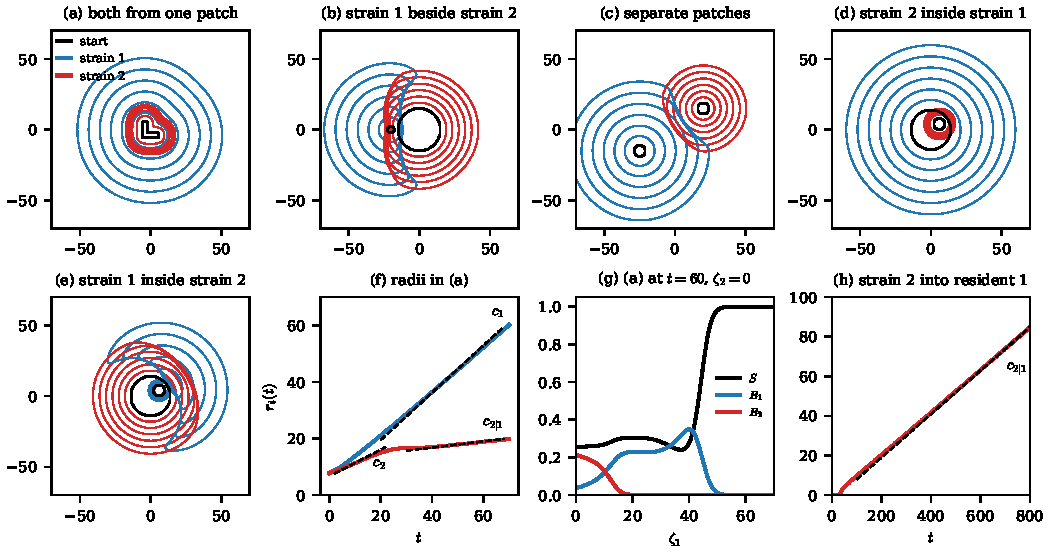
\includegraphics[width=\linewidth]{choFront}
\caption{The two-strain cholera model with spatial diffusion $d_1=1$, $d_2=1/4$, in the plane, with illustrative parameters: $\Lambda=\mu=0.1$, $\beta_1=1$, $\beta_2=1.2$, $\xi_i=\delta_i=1$, $\gamma_i=0.2$,  so $R_1\approx1.83$, $R_2=2$, $R_{2|1}\approx1.10$.
Panels (a)--(e): the fronts, meaning the level curves $B_1=0.01$ (blue) and $B_2=0.01$ (red), at $t=10,20,\ldots,60$; the black curves are the starting patches. (a) Both strains start from the same $L$-shaped patch. (b) Strain $1$ starts from a small disc beside a large disc of strain $2$. (c) The strains start from separate small discs, and each spreads into the disease-free state until they meet. (d) Strain $2$ starts from a small disc inside a large disc of strain $1$, and stays behind it. (e) Strain $1$ starts from a small disc inside a large disc of strain $2$, and escapes.
Panel (f): in (a), the front radius $r_i(t)=\sup\{|\zeta|:B_i(t,\zeta)\ge0.01\}$; the dashed lines have the slopes of the linear speeds $c=\inf_{\lambda>0}s(\lambda^2\mathcal D+M)/\lambda$, namely $c_1\approx0.84$, $c_2\approx0.47$, $c_{2|1}\approx0.11$. Strain $2$ moves into the disease-free state, at a slope approaching $c_2$, until strain $1$, which diffuses faster although it has the smaller reproduction number, has passed and lowered $S$; near $t=25$ the slope changes to about $c_{2|1}$, since strain $2$ now invades the resident equilibrium of strain $1$. Panel (g): the profiles in (a) at $t=60$ along $\zeta_2=0$, $\zeta_1\ge0$, show this: ahead $S=1$, behind the front of strain $1$ $S$ settles at $S_1^*=0.3$, and behind that of strain $2$ it falls toward $S_2^*=0.25$. Panel (h): the invasion in its pure form, on a half line, with the resident of strain $1$ everywhere and a small localized $B_2$; the position of $B_2=0.01$ has slope $0.1076$ on $400<t<800$, against the linear $c_{2|1}=0.1097$, and halving the mesh changes this by less than $0.001$.
Panels (a)--(e): $\zeta\in[-75,75]^2$, no-flux boundary, mesh $0.5$; (h): $\zeta_1\in[0,160]$, mesh $0.25$; explicit Euler.}
\label{fig:choFront}
\end{figure}

%=======================================================================
\subsection{Computational realization by conic optimization}
\label{s:spread-conic}
%=======================================================================

\beT[Convex feasibility certificates for the speed][][SpdQC]
In the setting of Proposition~\ref{t:spread}, for any $c>0$,
\[
c_*\le c
\qquad\Longleftrightarrow\qquad
\exists\,\lambda>0,\ w\gg0:\quad
\bigl(M+\lambda^2\mathcal D-c\lambda I\bigr)w\le0 .
\]
With $w_i=e^{u_i}$ and $u_1=0$, this is the convex feasibility problem in
$(\lambda,u)$
\[
M_{ii}+d_i\lambda^2-c\lambda+\sum_{j\ne i}M_{ij}e^{u_j-u_i}\le0,
\qquad i=1,\ldots,m ,
\]
and each accepted trial value comes with a certificate $(\lambda,w)$
verifiable by $m$ inner products.
\end{theorem}
\begin{proof}
$c_*\le c$ iff $g(\lambda)\le c\lambda$ for some $\lambda>0$, i.e.\
$s(M+\lambda^2\mathcal D)\le c\lambda$, i.e.\
$s\bigl(M+\lambda^2\mathcal D-c\lambda I\bigr)\le0$, the shift by
$-c\lambda I$ moving the spectrum rigidly. The shifted matrix is Metzler,
and for irreducible Metzler matrices $s(A)\le0$ is equivalent to the
existence of $w\gg0$ with $Aw\le0$ by Collatz--Wielandt. Dividing the $i$th
inequality by $w_i=e^{u_i}>0$ gives the displayed constraints, which are
convex in $(\lambda,u)$ because $M_{ij}\ge0$ for $j\ne i$; the normalization
$u_1=0$ removes the scaling freedom.
\end{proof}

Deciding whether a proposed
speed is achievable is a convex feasibility problem in $(\lambda,u)$, a
linear program in $w$ only once $\lambda$ is fixed, and a positive answer is
witnessed by a pair $(\lambda,w)$ that can be checked without any
eigenvalue computation: one forms $M+\lambda^2\mathcal D-c\lambda I$,
multiplies by $w$, and checks $m$ signs. Bisecting on $c$ then converges
to $c_*$; the problem is convex for fixed $c$ only, not jointly in $c$. Each verified feasible iterate provides a certified upper bound, whereas a failure of the solver certifies nothing, so a certified lower bound needs an infeasibility certificate.

% The code, random seeds, parameters and tolerances of this check must accompany the paper.
\medskip\noindent\textbf{Numerical check.} On $300$ random pairs
$(M,\mathcal D)$ with $M$ Metzler, $s(M)>0$, and sizes $2$ to $4$, the
second differences of $g$ on a grid of $400$ values of $\lambda$ were
nonnegative throughout, and every sampled sublevel set of $c$ was an
interval, as Proposition~\ref{t:spread} requires. On four further instances the
bisection of the theorem, which never computes a spectral radius, was
compared with direct minimization of
$c(\lambda)$ over a fine grid; the two agreed to $3\cdot10^{-4}$ or
better, the residual being the grid spacing of the direct method rather
than error in the bisection.

\beR[]
\label{r:spread-conic-scope}
The strong convexity of $g$ in Proposition~\ref{t:spread} is what makes the one-dimensional search
safe, and it is not automatic: it uses the convexity of the Perron root
in the diagonal entries, which is a property of Metzler matrices and
would fail for a general linearization. This is the same structural
hypothesis --- irreducible Metzler transversal block --- that underlies
the invasion certificates elsewhere in this paper, appearing here in the
different guise of making a wave-speed optimization tractable.
\eeR

